\chapter{Flow of Dry Water: consequences}
\section{Dos and Don'ts of the Bernoulli's equation}
The Bernoulli's equation is a much used and often abused concept in fluid mechanics. 
To see its power and its limitations let us work out a few examples. 
\subsection{Flow out of a hole}
\begin{marginfigure}
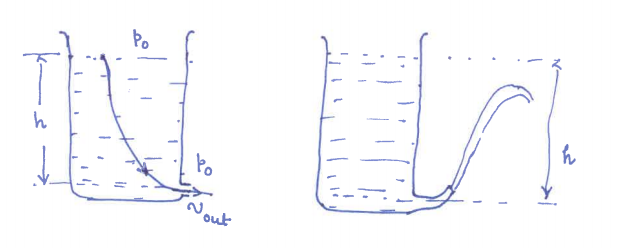
\includegraphics{figures/Toricelli.png}
\caption{Flow out of a hole at the bottom of a tank}
\end{marginfigure}
Take a water tank with a hole at its side near the bottom. 
If you open the hole what will be the velocity of the water coming out ?
You can work this out using Bernoulli's theorem. Consider a streamline from
 the surface of the water in the tank down to the hole and apply Bernoulli's equation to it.
Let us take the zero of the gravitational potential $\Psi$ at the surface of the water in the tank
where the velocity is zero.  
As the pressure at the two ends of the streamline is give by the atmospheric pressure the 
equation looks like:
\begin{equation}
\pzero = \pzero + \frac{1}{2}v^2_{\rm out} -  g h 
\end{equation}
which implies $v_{\rm out} = \sqrt{2gh}$. This is known as Toricelli's law. 
Note that you cannot get the rate at which water leaves the tank by just multiplying this velocity 
by the area of the hole. To quote Feynman~\cite{Feynman77}
`` The fluid velocities as the jet leaves the hole are not all parallel to each other but have components inward toward the center of the stream  
-- the jet is converging. After the jet has gone a little way, the contraction stops and the velocities do become parallel. So the total flow is the velocity times the area at that point. In fact, if we have a discharge opening which is just a round hole with a sharp edge, the jet contracts to 62 percent of the area of the hole. The reduced effective area of the discharge varies for different shapes of discharge tubes, and experimental contractions are available as tables of efflux coefficients.''
Clearly, everything that I have said above assumes that the tank is large enough or the hole
is small enough such that when the water 
flows out of it the height of the water in the talk changes slowly compared to the rate at which water flows out 
of the tank.  There are however bigger conceptual problem in applying Bernoulli's equation to this problem. 
If instead of letting the water out we added a discharge tube such that the water flowed upwards then if Bernoulli's equation were
correct water would rise to the level of water in the tank itself.  This simple experiment, which I am not going to do in class,
shows that water always falls short. This is because of the loss of energy due to viscous effects. 

\subsection{Bernoulli levitation}
\begin{marginfigure}
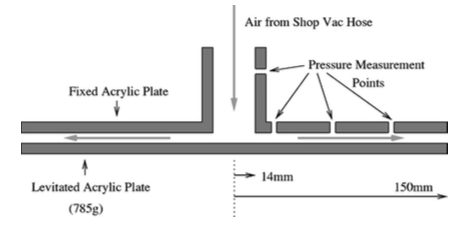
\includegraphics{figures/BernoulliLevitation.png}
\caption{A sketch of the experiment by Waltham et al.}
\label{fig:waltham}
\end{marginfigure}
\begin{marginfigure}
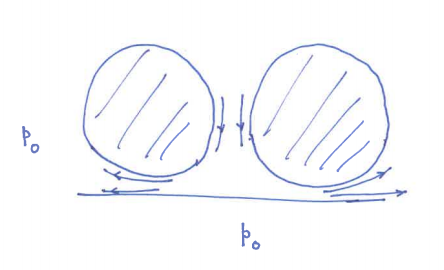
\includegraphics{figures/SommFingers.png}
\caption{A sketch of blowing at a piece of paper through your fingers. }
\label{fig:SommFinger}
\end{marginfigure}
A nice demonstration of the the Bernoulli's equation is given by Waltham et al\cite{waltham2003bernoulli}.
A pump forces air through a narrow horizontal channel as shown in \Fig{fig:waltham}. As the velocity
is increases the pressure decreases, this make the atmospheric pressure outside lift up the bottom plate. 
In the absence of the necessary equipment you can see a theorist's version of this experiment 
as was suggested by Sommerfeld~\cite{SomII}. Take a piece of light paper on a table. I have got the best effects
by using a square of toilet paper. Then blow at it through a small slit created between two of
your fingers. With a little bit of practice you can lift the paper up. It works better the lighter the
paper is.  If by some chance you have papers people used to roll up cigarettes you may have very good results. 
The flow comes down through the slit and then moves horizontal. 
\subsection{Can Bernoulli fly aeroplanes ?}
It is now natural to ask does the Bernoulli's equation describes, at least qualitatively, how aeroplanes get their lift ?
There are many places in the Internet, including webpages hosted by NASA and MIT that 
says yes. In truth the answer in no. It will take some time to explain. 
For the first half of this discussion I shall follow closely an 
article~\cite{babinsky2003wings} by Holger Babinsky.
\begin{marginfigure}
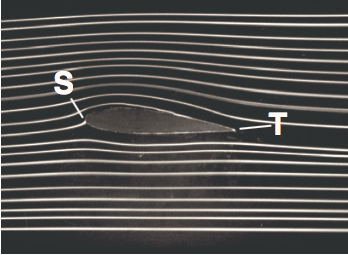
\includegraphics{figures/WingStreamlines.png}
\caption{Streamlines about the cross-section of a wing
visualized with smoke. Figure taken from the paper by Babinsky. }
\label{fig:WingStream}
\end{marginfigure}
The popular argument goes as follows: The typical shape of a wing it is curved 
on one side and flat on the other. The distance from the point at the front on 
the wind to its tail is greater if you follow the upper edge and less if you follow the 
lower edge. So you may argue that two fluid particles that follow two different
streamlines -- one just above and one just below the wing -- reaches the
tail at the same time. Hence the one above goes at faster speed. According
to Bernoulli's equation faster speed gives rise to lower pressure, hence 
there will appear lower pressure on the top of the wind and higher on the bottom. 
This explains the lift. This explanation is wrong on several counts 
\begin{enumerate}
\item First, Bernoulli's equation applies to individual streamlines, it does not
allow you to compare two different streamlines with each other. So the application
of Bernoulli's equation in the manner just described is essentially wrong. 
\item Second, you should ask why should the two fluid particles meet at the end of the
wing ? I do not know why. And real life observation show that they do not,
see for example the movie at 
\url{http://iopscience.iop.org/article/10.1088/0031-9120/38/6/001/data}
that accompanies the paper by Babinsky. In \Fig{fig:WingTopAndBottom} we show three snapshots
from the movie.
\begin{figure}
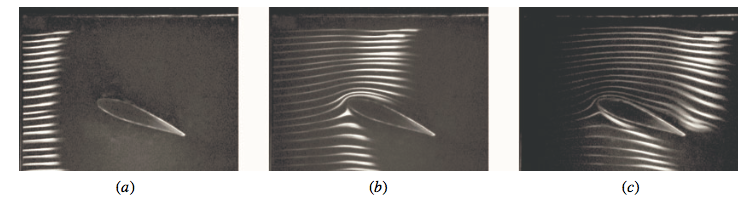
\includegraphics{figures/WingSpeedUpAndBottom.png}
\caption{Three snapshots of smoke particles flowing along 
a wing. Notice how the particles above reach the end of the wing
before the particles at the bottom. The statement that they should
reach the trailing end of the wing together is wrong. The figure is
taken from the paper by Babinsky.}
\label{fig:WingTopAndBottom}
\end{figure} 
\item You can generate a lift even in the case where two two sides have the same length. 
A typical example is that of a sail.
\end{enumerate}
\marginnote{
There are parts of Internet that debates whether Newton's laws or Bernoulli's equations
are responsible for the lift. This question itself is meaningless because Bernoulli's
equations are consequences of Newton's laws. Whatever we do in classical
mechanics is a consequence of Newton's laws. 
}
So, how does the aeroplane fly then ? At this moment I am not giving you an answer. 
Later in the course we hope to calculate the drag and the lift forces on a wing. 
It will then become clear exactly how and why planes fly. 
Nevertheless, not that in all our discussions about wing and flights so far we have ignored the role of viscosity. 
In this particular case viscosity plays a crucial role. The speed of the flow at any boundary
must be zero. This condition is imposed by the viscosity. The interaction between the
wing and the air is through viscous effects. You cannot understand flights unless you
understand viscous effects. The Euler equation and the Bernoulli equation which is a 
consequence of it does not contain viscous effects, hence they cannot describe either drag or lift. 
\section{A solution of Euler equation}
The steady Euler equation, in the absence of gravity, can be written in the following way:
\begin{equation}
(\curl\vv)\times\vv = -\grad\left\{\frac{p}{\rho} + \frac{1}{2}
v^2\right\}
\label{A2.2:SteadyEuler}
\end{equation}
This is clearly a non-linear equation, hence in general there can be
more than one solution. The form of the equation suggests that there
can be a solution such that 
\marginnote{
There is a systematic way of solving 
the eigenvalue problem in \Eq{A2.2:EigenCurl}.
By taking another curl and using $\dive\vv=0$ we obtain
\begin{equation}
\lap\vv + \Lambda^2 \vv = 0 \/,
\end{equation}
which is the vector wave-equation. This is solved by 
\begin{equation}
\vv = \frac{1}{\Lambda}\curl\curl(\nhat\psi) + \curl(\nhat\psi)
\end{equation}
where $\nhat$ is any fixed unit vector and $\psi$ is a scalar
function that satisfies the wave-equation
\begin{equation}
\lap\psi + \Lambda^2\psi = 0
\end{equation}
This was worked out by Chandrasekhar and Kendall~\cite{cha+ken57}.
}
\begin{equation}
\curl \vv = \Lambda \vv
\label{A2.2:EigenCurl}
\end{equation}
where $\Lambda$ is a constant. Clearly this satisfies the
incompressibility  constrant 
\begin{equation}
\dive \vv = 0 \/.
\end{equation}
(How will you show this ? ) If you substitute \Eq{A2.2:EigenCurl} in
\Eq{A2.2:SteadyEuler} the LHS side is zero. What about the RHS ? 
Can you show that it is zero too ? A different way to show that
\Eq{A2.2:EigenCurl} gives one solution of the Euler equation is to use
the vorticity equation that you derived in Exercise~\ref{Ex3}, Problem~\ref{prb3.1},
and consider the steady case $\partial_t \oo = 0$, in which case
we end up with
\begin{equation}
\curl(\oo\times\vv) = 0 \/,
\nonumber
\end{equation}
which is clearly satisfied by \Eq{A2.2:EigenCurl}.  So 
we have reduced the problem of finding a solution to the steady Euler
equation to a linear problem, that of finding a solution to the linear
equation \Eq{A2.2:EigenCurl}~\footnote{You need to be a little
  cautious here. Even if we manage to solve \Eq{A2.2:EigenCurl} we get
  only \textit{one} solution of the Euler equation. There may be many
  more. }. 
There is a wonderfully symmetric solution given by the following
expression
\begin{subequations}
\begin{align}
v_x(y,z) &=   A \sin \Lambda z + C \cos \Lambda y \\
 v_y(x,z) &=  B \sin \Lambda x +  A \cos \Lambda z \\
 v_z(x,y) &=  C \sin \Lambda y +  B \cos \Lambda x 
\end{align}
\label{A2.2:ABC}
\end{subequations}
%-------------------------------%
\begin{figure*}
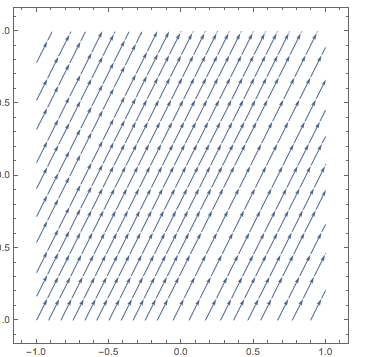
\includegraphics[width=0.23\linewidth]{figures/stream.png}
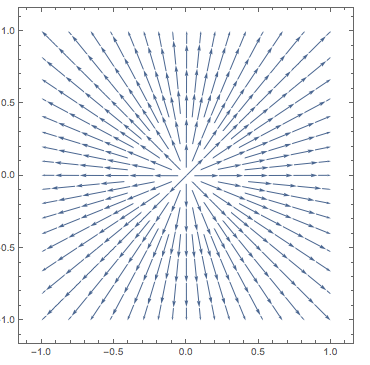
\includegraphics[width=0.23\linewidth]{figures/stream_source.png}
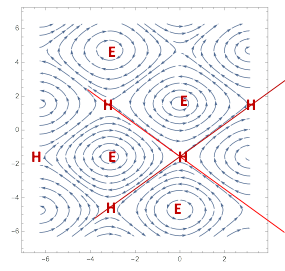
\includegraphics[width=0.23\linewidth]{figures/StreamAB.png}
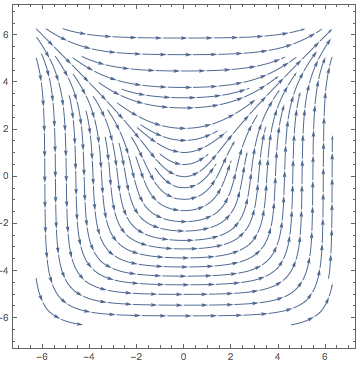
\includegraphics[width=0.23\linewidth]{figures/StreamHyp.png}
\caption{Few examples of streamlines. From left to right:
$v_x=1,v_y=2$, $v_x=x,v_y=y$, $v_x=\cos(y),v_y=\sin(x)$ and
$v_x=\cosh(y), v_y=\sinh(x)$. The second plot has non-zero divergence
at the origin -- a source. This cannot be the streamlines of an
incompressible flow. The third plot is particularly interesting. The
lines the separates the patch of circles from one another are called
separatrix. The center of the circle and the point where two
separatrices cross are \textit{fixed points} of this system -- points
where the velocities are zero, also called stagnation point in fluid
mechanics. There are two types of them -- ones around which the flow
looks elliptical, these are marked by {\bf E} and are called elliptic
points.  The others around which the flow looks hyperbolic, these are
marked by {\bf H} and are called hyperbolic points. 
Plotted using the {\tt StreamPlot} command of Mathematica.}
\label{fig:streamlines}
\end{figure*}
%-------------------------------%
 This is called the ABC (Arnold-Beltrami-Childress) flow. 
You can check this by direct substitution. There are
intriguing properties of this functions, some of which will be
explored in the exercises. 

\section{Streamlines}
Let us now revisit the streamlines.  We have a velocity
field $\vv(x,y,z)$ is space that is a constant in time. We want to
find the streamlines. Let us first consider the problem in two
dimensions. At any point $x,y$, the velocity has two components $v_x(x,y)$
and $v_y(x,y)$, which are both function of space. Let us write them as
$F(x,y)$ and $G(x,y)$. 
 To parametric equation for the streamlines can be
obtained by solving
\begin{subequations}
\begin{align}
\frac{dx}{dt} &= v_x(x,y) = F(x,y ) \\
\frac{dy}{dt} &= v_y(x,y) = G(x,y)
\end{align}
\label{A2.2:2dstream}
\end{subequations}
\marginnote{An integral of motion of a dynamical system is
  something that remains constant as the system evolves.}
These equations can be considered a two coupled ordinary
differential equations (ODEs). The functions $F$ and 
$G$ can in general be nonlinear.  The problem is then 
an initial value problem with the initial position of the fluid
particle as the point where the streamline starts. 
 You can think about several simple
cases where these equations can be easily solved. 

But we are not going to discuss those special cases now -- they can be
found in the appendix of this chapter. 
I have plotted several typical examples of streamlines in
\Fig{fig:streamlines} in two dimenions. 
\subsection{The general case}
\begin{marginfigure}
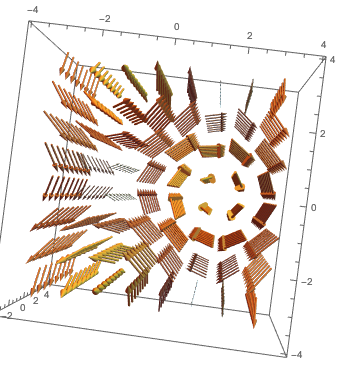
\includegraphics[width=5cm]{figures/ABC1.png}\\
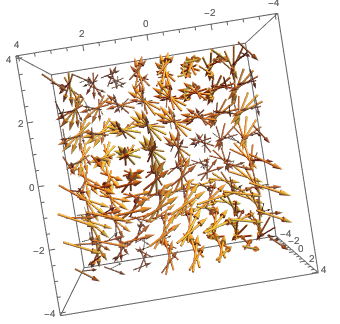
\includegraphics[width=5cm]{figures/ABC2.png}\\
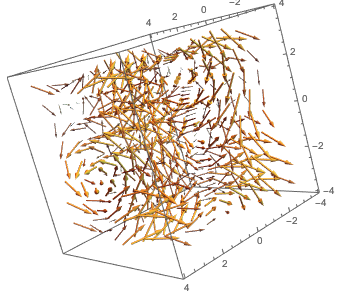
\includegraphics[width=5cm]{figures/ABC3.png}
\caption{Three graphical representations of the ABC flow. In all the
  three $\Lambda=1$. In the top one $C=0$. The second and the third
  are two different views of vector plot of the flow}
\label{fig:ABC}
\end{marginfigure}
To think about the general case think about the problem in the
following way. \Eq{A2.2:2dstream} forms a two dimensional dynamical
system. There are certain properties that $F$ and $G$ must satsify, in
particular, they must be such that the Bernoulli's equation
holds. That implies that there in one \textit{integral of motion} 
-- the energy. This sets
certain constraint on the system. In particular, in two dimension, one
constraint implies that the motion must remain on a curve. This means
that there exists a transformation (in general nonlinear), 
from $x,y$ to $\xi,\eta$ such that the motion happens along the curve
$\xi = \text{constant}$. This means that \Eq{A2.2:2dstream} is an 
\textit{integrable system}. The other coordinate $\eta$ must do one of
the two things : (a) it can go away to infinity (open streamlines) (b)
it must be a periodic variable, like an angle. 

\subsection{In three dimensions}
Why did I spend so much time in this section on a problem that seem
pretty obvious ? Thinking in a simple way, in a steady flow fluid
particles follow streamlines. As one fluid particle cannot go in two
different paths and must go along exactly one path, the solution to
\Eq{A2.2:2dstream} must exist and must be unique. Actually,
irrespective of the number of dimensions, it should hold in three
dimensions too. And indeed it does, streamlines in three dimensions
are unique and they exist but they are not always
\textit{integrable}. Revisiting the argument about an integral of
motion, when we are in three dimensions we have three equations with
one constraint (the integral of motion). This confine a streamline to
a surface, not a line. This fact has a major implication. For example,
the streamline can now cover this surface \textit{ergodically} -- it
can come as visit almost every point on this surface, like wrapping a
thread of wool on a ball -- of course without ever intersecting
itself. Secondly, two streamlines that initially are very close to
each other can go away from each other \textit{very fast} -- in
particular exponentially fast. Let us start with two points in $x,y,z$
given by $\rnot$ and $\rnot+\Delta \rr$.
As we follow the two streamlines that evolves from these two points we
may find that the distance $\Delta \rr$ grows exponentially fast in
time, e.g., as $\exp(\lambda t)$ where $\lambda$ is positive. 
This is a typical feature of \textit{chaotic} systems -- sensitive
dependence on initial conditions. And the exponent $\lambda$ is called
the largest Lyapunov exponent. So the streamlines in three dimensions
can be chaotic -- not so in two dimensions. An example of chaotic
streamlines is actually the ABC flow~\eq{A2.2:ABC} for $A=B=C=1$. 
It is not chaotic if any of the three constants are zero. The beauty
and complexity of this problem has been explored in several papers, I
suggest you start with the one by Dombre and his collaborators~\cite{dom+fri+hen+gre+sow86}.   
\section{Back to conservation laws}
Let us now revisit the conservation law we derived in the last
lecture. We noted that for any conserved density variable $\rho$ we
can write down a conservation law of the general form
\begin{marginfigure}
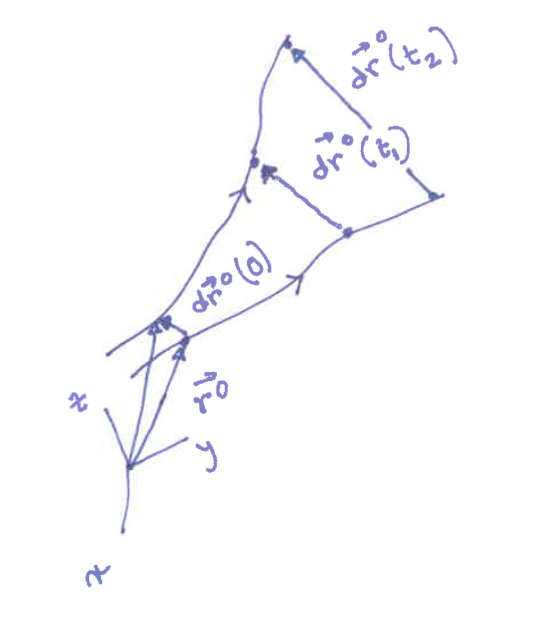
\includegraphics{figures/Lyapunov.png}
\caption{Two streamlienes that are very close to each other near
  $\rnot$ diverges away from each other exponentially fast. The
  exponent give the largest Lyapunov exponent. This is a typical
  signature of chaos.}
\label{fig:Lyap}
\end{marginfigure}
\begin{equation}
\partial_t \rho + \dive \JJ = 0
\end{equation}
We have already applied this to mass and obtained the continuity
equation. Let us try to apply this to the next conserved quantity
momentum. The momentum density function 
$\PP = \rho\vv$. But momentum is not conserved in the same way that
mass is. If we consider a small volume of the fluid  -- this time not a
fluid particle but a fixed volume $\delta V$ in space -- then the
momentum of this volume changes in two ways. One, the one we are
already familiar with is the divergence of all stresses acting on this
volume. As the divergence of stresses constitute a force they
contribute to the rate-of-change of momentum to this volume. So the
conservation equation now looks like 
\begin{equation}
\partial_t P_{\alpha} - \partial_{\beta}\sigma_{\alpha\beta} +
\dive\left(\parbox{2cm}{flux of  $P_{\alpha}$}\right) = 0 
\label{A2.2:mflux1}
\end{equation}
What is the flux vector of a component of momentum ? Remember, the
flux of any quantity due to the flow is the same quantity multiplied
by the velocity. The flux of a scalar dentsity is a first rank tensor
-- a vector. The flux of a vector quantity is, you guessed it, a
second rank tensor. The flux of momenum is given by 
\begin{equation}
\Pi_{\alpha\beta} = v_{\beta}P_{\alpha} = \rho v_{\alpha}v_{\beta} 
\label{A2.2:momflux}
\end{equation}
Substituting this back in \Eq{A2.2:mflux1} we obtain
\begin{equation}
\partial_t (\rho v_{\alpha}) + \partial_{\beta}\left[ \rho
  v_{\alpha}v_{\beta} - \sigma_{\alpha\beta} \right] = 0
\label{A2.2:EAgain}
\end{equation}
Can you see that this is the Euler equation reborn ? 
\begin{Exercise}
\label{Ex3}
\Question
\label{prb4.1}
{\bf Helicity}\\
The helicity density, at a point in  a flow is given by 
\begin{equation}
h = \oo\cdot\vv
\end{equation}
where the flow velocity is given by $\vv$ and the vorticity $\oo =
\curl \vv$. 
Calculate the total helicity $\mathcal{H}$ of the ABC flow 
defined by 
\begin{equation}
\mathcal{H} = \int_{-\pi}^{\pi}dx \int_{-\pi}^{\pi}dy
\int_{-\pi}^{\pi}dz (\oo\cdot\vv) \/,
\end{equation}
for $A=B=C=1$. 
\Question
\label{prb4.2}
Using the continuity equation, show that \Eq{A2.2:EAgain}
is the Euler equation. 
\Question
\label{prb4.3}
{\bf The Venturi tube} \\
A sketch of the Venturi tube in given in \Fig{fig:venturi}. Using the
continuity equation and the Bernoulli's equation show that the
flowrate through the tube is given by 
\begin{equation}
Q = \frac{A_2}{1-(A_2/A_1)^2}\sqrt{2gh}
\label{A2.2:venturi}
\end{equation}
where $g$ is the gravitational acceleration and rest of the symbols
are explained in the caption of \Fig{fig:venturi}. In practice the
formula is wrong; the RHS must be multiplied by a ``fudge factor'', C
which must be determined experimentally. 
\end{Exercise}

\section{Measurement of flow velocity}
Unfortunately this course is a totally theoretical one, while fluid
dynamics is a subject that is intimately connected with experiments. I
have neither the skill nor the time to go into measurement of flow
properties in any detail. Let me just touch on few methods that are
commonly used to measure flow velocities. 
\subsection{Venturi tube and Pitot tube}
\begin{marginfigure}
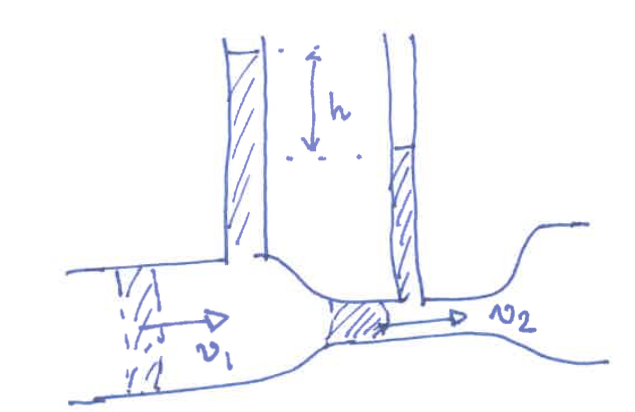
\includegraphics{figures/venturi.png}
\caption{A sketch of Venturi tube. The flowrate through the tube is
  given by $Q$, in \Eq{A2.2:venturi}. The area of the wider part of
  the tube is $A_1$ and the area of the narrower part is $A_2$. The
  difference is height of the pressure heads is $h$. }
\label{fig:venturi}
\end{marginfigure}
Notice that if the fluid passes through a constriction its velocity
should increase (why ?) and this means that locally the pressure will
decrease. By measuring this drop in pressure through the Bernoulli's
equation you can measure the flow velocity. 

A very clever generalisation of this idea is implement in Pitot
tube. In its simples avatar it is just a bent tube. If you put it in a
river (according to rumours Pitot used the Seine) the level of water
that rises in the tube is determined by the ballance between the
pressure in the flow and the atmospheric pressure. The pressure in
turn depends on the flow velocity and thus the level upto which the
water rises depends on the flow velocity. If you put down a bent tube
in a river and turn in around the height up to which water rises in
the tube changes depending on whether the hole faces the flow
direction or not. A more sophisticated version is a design where there
are two holes one at the end and one at the side. The difference in
the pressure head, $h$, in these two channels give the flow velocity as
$v = C\sqrt{2gH}$. Notice that it must be multiplied by a ``fudge
factor'' of $C$ called the coefficient of velocity.  We faced similar
factors while dealing with flow out of a hole too. 
\begin{marginfigure}
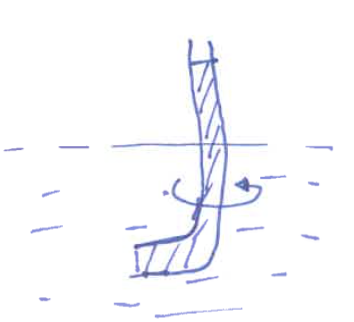
\includegraphics{figures/pitot1.png}\\
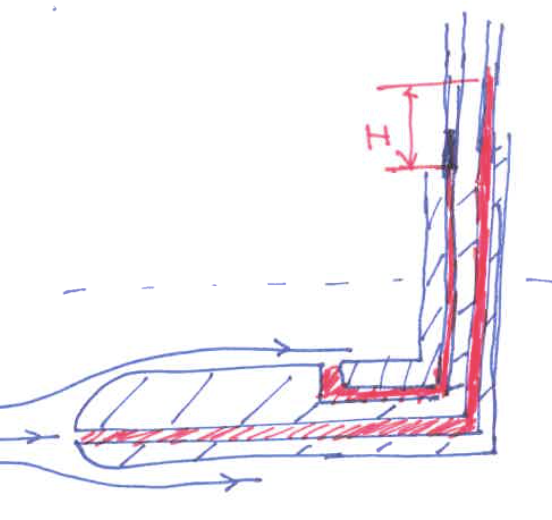
\includegraphics{figures/pitot2.png}
\caption{Sketch of the Pitot tube.}
\label{fig:pitot}
\end{marginfigure}
\subsection{Hot air anemometer}
The fact that air cools down a hot object can be used to measure the
speed of air. This is the principle of a hot wire anemometer. The
idea is that you control the heating of a wire by an electrical
circuit to hold its temperature constant. This implies that the rate
at which electrical energy is dissipated is the same rate at which it
is carred away by the wind. To quote from Encyclopedia Britannica
``In the most common type of hot-wire anemometer,
 the constant-temperature type, power is increased to maintain a
 constant wire temperature. The input power to the hot wire is the
n a measure of airspeed, and a meter in the electrical circuit of the 
hot wire can be calibrated to indicate airspeed. This device is useful
 for very low airspeeds, below about 5 miles (8 km) per hour.''
These are most commonly used in wind tunnels and abroad aircrafts. 
I enthusiastically recommend the Wikipedia article on anemometers:
\url{https://en.wikipedia.org/wiki/Anemometer}. 
\subsection{Particle image velocimetry}
This is one of the modern methods of measuring flow velocities that
has revolutionasied research in fluid mechanics. The idea is that 
many small sphere with almost the same density as the fluid itself is
released in the fluid. These are then tracked by very fast cameras. By
comparing the position of the particles from one frame to another
their velocities are measured. What you get is essentially very close
to the Lagrangian velocity of many particles which allows you to map
out the Eulerian velocity field too at that instant. You get as close
to Lagrangian velocity as you can match the density of the particles
with that of the fluid. The smaller the particles are, more accurate
are the measurements. 
\section{Kelvin's theorem}
We are now at the end of our discussion of flow of ``dry water''. 
There is one very important result that I need to discuss. This states
that
\begin{thm-non}
In inviscid fluid the flux of vorticity through an open Lagrangian surface
remains constant in time.
\end{thm-non}
Before proving it let us try to understand its content. First note
that it says ``Lagrangian surface'', what does that mean ? It means
the following:  at time $t=0$ you mark a surface, i.e., you mark every
point on the surface; then calculate the flux of vorticity through
this surface.  Then as time evolves that Lagrangian particles move
elsewhere, as they do the surface changes but the flux of vorticity
through this ``new'' surface is the same as it was through the ``old''
surface. So mathematically we restate the theorem as 
\begin{thm-non}
In inviscid fluid 
\begin{equation}
D_t \int_S \oo\cdot\nhat dS = 0 
\label{A2.2:Kelvin}
\end{equation}
where $D_t \equiv  \partial_t + \vv\cdot\grad$ is the material
derivative. 
\end{thm-non}
 Note next that the theorem say, \textit{open surface}. From Stokes
theorem, you know that the flux of any vector field through an open
surface is equal to its line integral over the line that bounds the
surface. So an alternative statement of the Kelvin's theorem is 
\begin{thm-non}
In inviscid fluid
\begin{equation}
D_t \oint_{\Gamma} \oo\cdot\dL = 0 
\end{equation}
where $D_t \equiv = \partial_t + \vv\cdot\grad$ is the material
derivative.  
\end{thm-non}
The integral of vorticity along a closed line is called circulation
\begin{equation}
 C = \oint_{\Gamma} \oo\cdot\dL \/.
\end{equation}
With this definition we can restate Kelvin's theorem as 
\begin{thm-non}
In inviscid fluid the circulation of any closed Lagrangian
line remains constant in time. 
\end{thm-non}
Note next that this theorem is true only for inviscid fluid, i.e., dry
water. So far in this chapter we have seen that most conclusion that
we draw from our theory of dry water are quantitatively wrong -- most
of the time we have to include an arbitrary factor to fix it to match
experiment. Do we need to do something similar for the Kelvin's
theorem when we deal with real fluids ? I do not/can not answer this
question at this point, but just want to raise it. 
\subsection{Potential flows}
Note a particularly interesting consequence of this theorem. If to
begin with vorticity was zero everywhere in a domain then in an
inviscid fluid it will reamin so at all future times. This makes it
particularly interesting to consider the case of \textit{irrotational
  flows} where
\begin{equation}
\curl \vv = 0 \quad \text{everywhere.}
\end{equation}
\marginnote{
A word of warning. If we assume an initially irrotational flow
everywhere in a real fluid you are the flow will not necessarily
remain irrotational in future. Vorticity is going to be generated, due
to viscous effects mostly near the boundary of the flow. The vorticity
thus generated will diffuse into rest of the flow. We shall spend
some time discussing this mathematically few chapters later. 
}
\marginnote{
The \Eq{A2.2:irro} is the same equation satisfied by a static electric field
in a domain where the charges are confined only the boundary of the
domain. For example inside a capacitor. Or inside a metal box whose
different faces are raised to different potential. \Eq{A2.2:potential}
is then the equation satisfied by the electrostatic potential. If you
have had a typical undergraduade course on electromagnetism, something
at the level of Griffith's book~\cite{Griffiths1962introduction} you already know quite a lot about
this problem.
}
For irrotational and incompressible fluid the equation of motion are
given by 
\begin{equation}
\dive \vv = 0 \quad\text{and}\quad \curl\vv = 0  \/.
\label{A2.2:irro}
\end{equation}
As the curl of velocity is zero, we can define a potential function
$\psi$ such that 
\begin{equation}
\vv = - \grad \psi
\end{equation}
because the curl of any gradient is zero. 
The potential for velocity then satisfies the equation
\begin{equation}
\lap \psi = 0 \/.
\label{A2.2:Laplace}
\end{equation}
This is called Laplace's equation. Remarkably, we have now reduced the
problem to solving a partial differential equation for a scalar
field. This equation is also called the potential equation and the
velocity that is a solution of such an equation the \textit{potential
  flow}.  If this where a traditional fluid mechanics course, we shall
now spend quite a lot of time solving the potential equation in all
its glory. The necessary mathematics is beautiful and important, but
is not of much use in reality because real flow are not potential at
all. Except in one very important case. Often the real flow about a
real wing can be thought about as two flows, one outer -- somewhat
away from the wing -- that is indeed irrotational and one inner --
quite close to the wing (boundary layer) -- that is controlled by the
viscous effects. To find a complete solution these two solutions must
be \textit{matched} with each other. The solution of potential flow
problems then do become important.  I shall come back to the potential
flows when I need them, but now I shall concentrate on the viscous
effects starting with the next chapter. 





%----------------------------------------------------------------------------------------
%----------------------------------------------------------------------------------------
\newpage
\section*{Summary of Act 2}
\begin{thm-non}
The equation of motion of a fluid with constant density, 
flowing under gravity, is given by the Euler equation
\begin{equation}
\partial_t \vv + \vv\cdot\grad\vv = -\frac{\grad p}{\rho}+\ggg   \/,
\nonumber
\end{equation}
with the incompressibility constraint
\begin{equation}
\dive \vv = 0 \/,
\nonumber
\end{equation}
if we ignore the viscous forces.
Here $\vv$ is the velocity, $p$ the pressure,
 $\rho$ the density, and $\ggg$ the gravity. 
\end{thm-non}
From this we can derive the Bernoulli's theorem which states that 
\begin{equation}
\vv\cdot\left\{ \frac{p}{\rho} + \Psi + \frac{1}{2}v^2\right\} = 0
\nonumber
\end{equation}
in a steady flow. Here $\ggg = -\grad\Psi$, i.e., $\Psi$ is the gravitational potential.   
 
\begin{thm-non}
If $\rho$ is a conserved density variable and $\JJ$ is its current then they 
together satisfies the local conservation law
\begin{equation}
\partial_t \rho + \dive \JJ = 0 
\nonumber
\end{equation}
\end{thm-non}
A consequence of this theorem and the fact that mass is conserved is the continuity equation
\begin{equation}
\partial_t \rho + \dive(\rho\vv) = 0
\end{equation}
where $\rho$ is the mass density and $\vv$ is the velocity of the flow. 
This is true irrespective of whether we consider incompressible or
compressible fluids. 
